\documentclass[11pt,letterpaper]{article}

\usepackage[margin=1in]{geometry}
\usepackage{amsmath,amssymb,amsfonts}
\usepackage{graphicx}
\graphicspath{{figures/}}
\usepackage{booktabs}
\usepackage{hyperref}
\usepackage{caption}
\usepackage{subcaption}
\usepackage{enumitem}
\usepackage{setspace}
\onehalfspacing

\title{Modeling and Simulation of a Pan-Tilt Camera\\
Based on the Pinhole Model}
\author{Your Name\\
ECE 5240 / MAE 5810 Robot Perception\\
Instructor: Silvia Ferrari}
\date{\today}

\begin{document}
\begin{titlepage}
\maketitle
\thispagestyle{empty}
\vfill
\begin{center}
Formula-corrected report draft.\\
Results describe the existing synthetic implementation.\\
Real-image validation and additional parameter sweeps remain future work.
\end{center}
\vfill
\end{titlepage}

\begin{abstract}
This report presents a mathematical model and simulation of a controllable pan-tilt (PT) camera based on the pinhole camera model. The implementation captures the dependence of image-plane measurements and the ground field-of-view (FOV) on the camera's orientation. Static obstacles are incorporated through a line-of-sight (LOS) visibility test. Numerical experiments validate the projection geometry and FOV membership, and a noise study confirms the population radial RMS under additive Gaussian measurement noise. A consistent rotation convention, positive-depth FOV gate, and position-only measurement equation are specified. Analytic sensitivity and height--area relations are derived, but their dedicated numerical validation remains future work. Synthetic consistency is distinguished from physical-camera validation.
\end{abstract}

\section{Introduction}
A controllable pan-tilt (PT) camera can be used to monitor a two-dimensional workspace $\mathcal{W} \subset \mathbb{R}^2$ over a time interval $(T_0,T_f]$. The position of a point target is denoted
\begin{equation}
\mathbf{x}_T = \begin{bmatrix} x_T & y_T \end{bmatrix}^T \in \mathcal{W}.
\label{eq:xT}
\end{equation}
The camera possesses a dynamic and bounded field-of-view $\mathcal{S}(t) \subset \mathcal{W}$, and obtains a measurement of the target at time $t$ only when $\mathbf{x}_T(t) \in \mathcal{S}(t)$. Pan rotates the ground footprint, while tilt can change its shape and area. Geometric FOV membership is necessary but is not sufficient for a measurement when LOS is obstructed.

This project implements a simulation of the PT camera based on the course handout \textit{Pinhole Camera Model and Field-of-view (FOV)}\cite{handout}, within the scope of the midterm assignment\cite{midterm}. The simulation demonstrates the dependence of measurements and FOV geometry on sensor orientation, and incorporates environmental occlusion. The remainder of the report is organized as follows. Section~\ref{sec:model} presents the mathematical model. Section~\ref{sec:sim} describes the simulation design. Section~\ref{sec:results} shows the experimental results. Section~\ref{sec:analysis} analyzes how the model captures the required dependencies. Conclusions are given in Section~\ref{sec:conclusion}.

\section{Mathematical Model of the PT Camera}
\label{sec:model}

\subsection{Pinhole Geometry and Coordinate Frames}
Based on the pinhole camera model, the lens is symmetric about an optical axis. Images of the workspace are projected onto a virtual image plane perpendicular to the optical axis and located at a distance $\lambda$ (the focal length) from the pinhole. A camera-fixed frame is defined with its origin at the pinhole, the $z$-axis aligned with the optical axis, the $x$-axis parallel to the $XY$-plane, and the $y$-axis obtained by the right-hand rule.

Let $C=[C_x,C_y,C_z]^T$ be the camera center and $X_T=[x_T,y_T,0]^T$ a ground target, both in the world frame. Define $R_{WC}$ as the camera-to-world rotation. A right-handed pan rotation about world $Z$ is followed by tilt about the intermediate $x$ axis:
\begin{equation}
R_{WC}=R_z(\psi)R_x(\phi),
\label{eq:rotation}
\end{equation}
where the active rotation matrices are
\begin{equation}
R_z(\psi)=\begin{bmatrix}
\cos\psi&-\sin\psi&0\\\sin\psi&\cos\psi&0\\0&0&1
\end{bmatrix},\quad
R_x(\phi)=\begin{bmatrix}
1&0&0\\0&\cos\phi&-\sin\phi\\0&\sin\phi&\cos\phi
\end{bmatrix}.
\end{equation}
Thus $R_{CW}=R_{WC}^T=R_x(\phi)^TR_z(\psi)^T$. In terms of the passive matrices printed in the handout, $R_\phi=R_x(\phi)^T$ and $R_\psi=R_z(\psi)^T$, the same world-to-camera transformation is $R_{CW}=R_\phi R_\psi$, without further transposes. This explicit definition avoids mixing active and passive conventions. At $\phi=\pi$ the camera looks vertically down; at $\phi=140^\circ$ and $\psi=0$ it looks downward and toward negative world $Y$.

\subsection{Projection onto the Virtual Image Plane}
A 2-D frame $(x_p,y_p)$ is embedded in the virtual image plane, with its origin at the intersection of the optical axis and the image plane. The projection of a target $\mathbf{x}_T$ onto this frame is
\begin{equation}
\mathbf{p}_T = \lambda \begin{bmatrix} q_x / q_z \\ q_y / q_z \end{bmatrix} \triangleq \begin{bmatrix} p_x \\ p_y \end{bmatrix},
\label{eq:projection}
\end{equation}
where the target position relative to the camera-fixed frame is
\begin{equation}
\mathbf{q}_T = R_{WC}^{T}(X_T-C) \triangleq \begin{bmatrix} q_x \\ q_y \\ q_z \end{bmatrix},
\label{eq:qT}
\end{equation}
where $C$ denotes only the camera center. The code stores points as rows; \texttt{(points - position) @ rotation()} is the row-vector equivalent. Image-plane coordinates have physical length units, not pixels.

\subsection{Field-of-View Condition}
The projection of the FOV $\mathcal{S}(t)$ onto the virtual image plane is a rectangle of the same size as the image sensor. Let $a$ and $b$ denote the width and height of the sensor. A target lies inside the camera FOV if and only if its image-plane projection lies inside the sensor:
\begin{equation}
\mathbf{x}_T(t) \in \mathcal{S}(t) \quad \Leftrightarrow \quad
q_z>0\quad\text{and}\quad \mathbf{p}_T \in \left[-\frac{a}{2},\frac{a}{2}\right] \times \left[-\frac{b}{2},\frac{b}{2}\right].
\label{eq:fov}
\end{equation}
For an image corner $d_i^C=[\pm a/2,\pm b/2,\lambda]^T$, the world ray is $d_i^W=R_{WC}d_i^C$. The ground intersection is
\begin{equation}
P_i=C+t_i d_i^W,\qquad t_i=-\frac{C_z}{(d_i^W)_z}.
\end{equation}
For $C_z>0$, a finite forward intersection requires $(d_i^W)_z<0$. Four such intersections yield the footprint. A corner ray that does not point downward is marked unavailable; a bounded quadrilateral must not be assumed near the horizon.

\subsection{Measurement Equation}
The current implementation measures image position only, not the full position--velocity vector in the handout. Let $v_k$ be true when a target satisfies the positive-depth FOV condition and its sight segment is unoccluded. The implemented model is
\begin{equation}
\mathbf{z}_k=\begin{cases}
\pi(q_k)+\epsilon_k,&v_k=1,\\
\emptyset,&v_k=0,
\end{cases}
\qquad \epsilon_k\sim\mathcal{N}(0,\sigma^2 I_2),
\label{eq:measurement}
\end{equation}
where $\pi$ is Eq.~\eqref{eq:projection}. The output is two-dimensional. Unavailable observations are represented by \texttt{NaN} and a validity mask, rather than a zero position.

\subsection{Implemented Extensions}
The open sight segment is $C+t(X_T-C)$, $0<t<1$. An axis-aligned solid box blocks a target when this segment intersects the box. A slab test intersects the admissible parameter intervals across all three axes. Noise is applied only after ideal FOV and LOS selection and does not alter the visibility decision. The assumed independent Gaussian noise is not a model of illumination or detection failure, and its parameters have not been calibrated against real images.

\section{Simulation Design and Implementation}
\label{sec:sim}
The simulation is implemented in Python. The camera uses a focal length of $\lambda = 0.02$\,m and a sensor of size $0.036\,\text{m} \times 0.024\,\text{m}$. In the reported experiments the camera is placed at a height of 8\,m above the ground plane $Z=0$. Four static point targets and one axis-aligned solid-box obstacle are used. All parameters are illustrative assumptions rather than physical-camera calibration. The core projection, FOV membership test, and occlusion check are implemented in \texttt{camera.py}. Result figures are generated by \texttt{explain\_run.py}.


\begin{table}[htbp]
\centering\small
\caption{Parameters used for the existing experiments.}
\begin{tabular}{ll}\toprule
Quantity & Value\\\midrule
Camera center, default pan/tilt & $(0,0,8)$ m; $0^\circ/140^\circ$\\
Targets 0, 1 & $(-2,-5,0)$, $(0,-8,0)$ m\\
Targets 2, 3 & $(3,-10,0)$, $(1,-4,0)$ m\\
Box lower/upper corners & $(-1,-5,0)$ / $(1,-3,4)$ m\\
Pan sweep & $-60^\circ$ to $60^\circ$, step $1^\circ$\\
Noise experiment pose & Same center; pan $0^\circ$, tilt $180^\circ$\\
Coordinate noise $\sigma$ & $0,0.02,0.05,0.1,0.2,0.5$ mm\\
Noise samples and seed & $10{,}000$/condition; seed $4810$\\\bottomrule
\end{tabular}
\end{table}
The four existing automated checks cover known downward-view projections and points behind the camera, footprint-corner reprojection, selected occlusion cases, and noise statistics. They passed in the current code. These checks are limited synthetic verification, not validation of a physical camera. The animation uses prescribed poses rather than motor-driven trajectories.

\section{Results}
\label{sec:results}

\subsection{Scene and FOV Visualization}
Figure~\ref{fig:scene} shows a representative scene. The left panel displays the ground footprint of the camera FOV together with the four targets (green if both inside the FOV and unoccluded; red otherwise) and the rectangular obstacle. The right panel shows the corresponding image-plane measurements in millimetres. At the default pose all four points satisfy the FOV gate, but only targets 0 and 2 remain visible, at approximately $(-4.282,-2.809)$ and $(4.779,4.011)$ mm. Target 3 is on the box boundary at ground level with solid material above it; this is not a clean separate-target occlusion scene. Future experiments should place targets outside obstacle volumes. The current scene is retained here to match the actual existing output.

\begin{figure}[htbp]
    \centering
    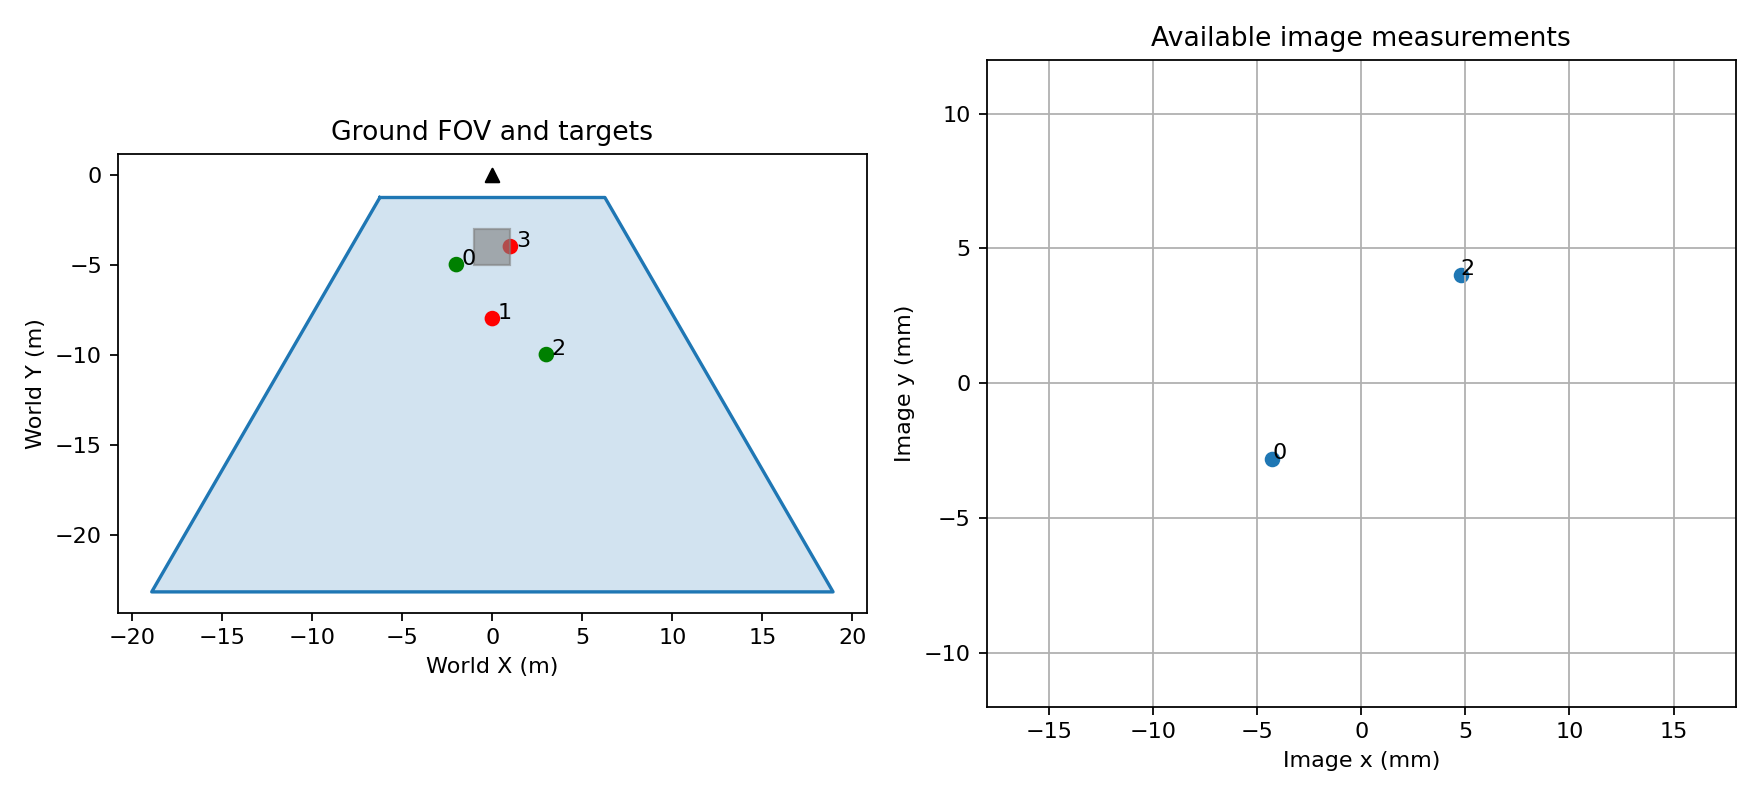
\includegraphics[width=0.92\textwidth]{01_scene.png}
    \caption{Scene visualization. Left: ground FOV footprint with visible (green) and unavailable (red) targets. Right: corresponding image-plane measurements.}
    \label{fig:scene}
\end{figure}

\subsection{Dependence on Pan Angle}
Figure~\ref{fig:pan} reports the number of targets that lie inside the geometric FOV and the number that remain visible after the occlusion test, as the pan angle varies from $-60^\circ$ to $+60^\circ$ in $1^\circ$ increments (121 samples). The gap is the number of occluded targets among those currently inside the FOV. With the camera center, targets and obstacle fixed, pan changes FOV selection but not the world-space LOS intersection for any particular target. A separate occluder or target-motion experiment is needed to isolate changes in LOS geometry.

\begin{figure}[htbp]
    \centering
    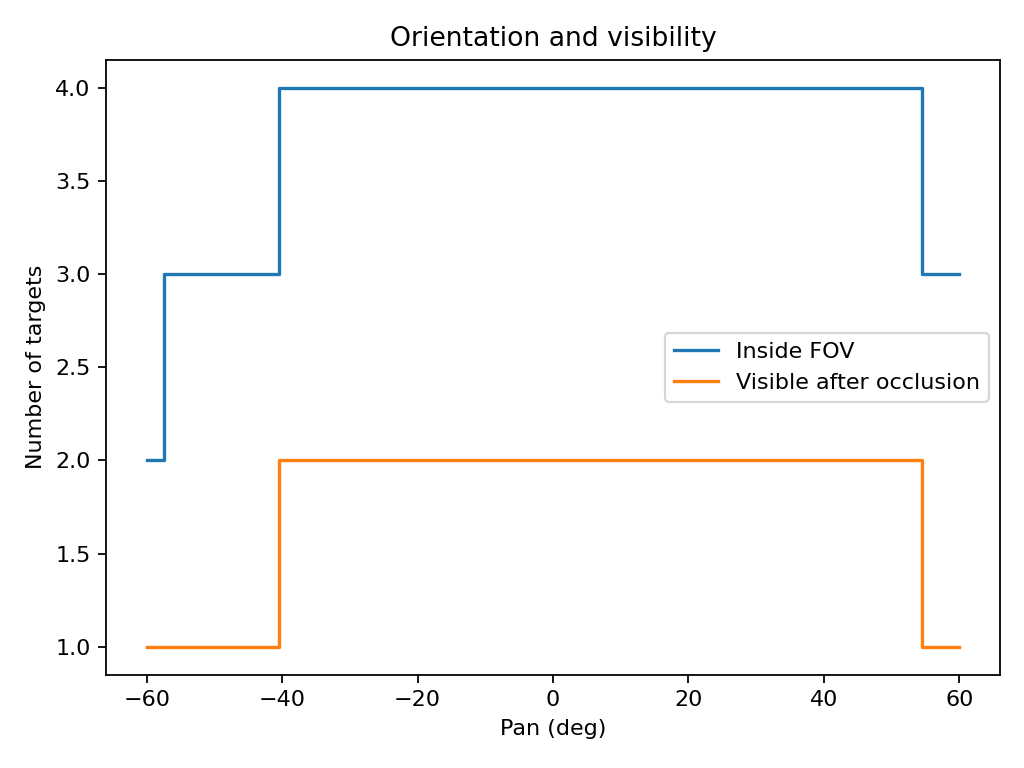
\includegraphics[width=0.78\textwidth]{02_pan.png}
    \caption{Number of targets inside the geometric FOV versus number remaining visible after occlusion, as a function of pan angle.}
    \label{fig:pan}
\end{figure}

\subsection{Noise Model Validation}
Additive zero-mean Gaussian noise with standard deviation $\sigma$ was applied to the image-plane coordinates of visible points. Figure~\ref{fig:noise} compares the simulated radial root-mean-square error against the population RMS value $\sqrt{2}\sigma$. The close agreement supports the assumed noise-generation and error-calculation steps; it does not verify the rotation matrices or real-camera accuracy.

\begin{figure}[htbp]
    \centering
    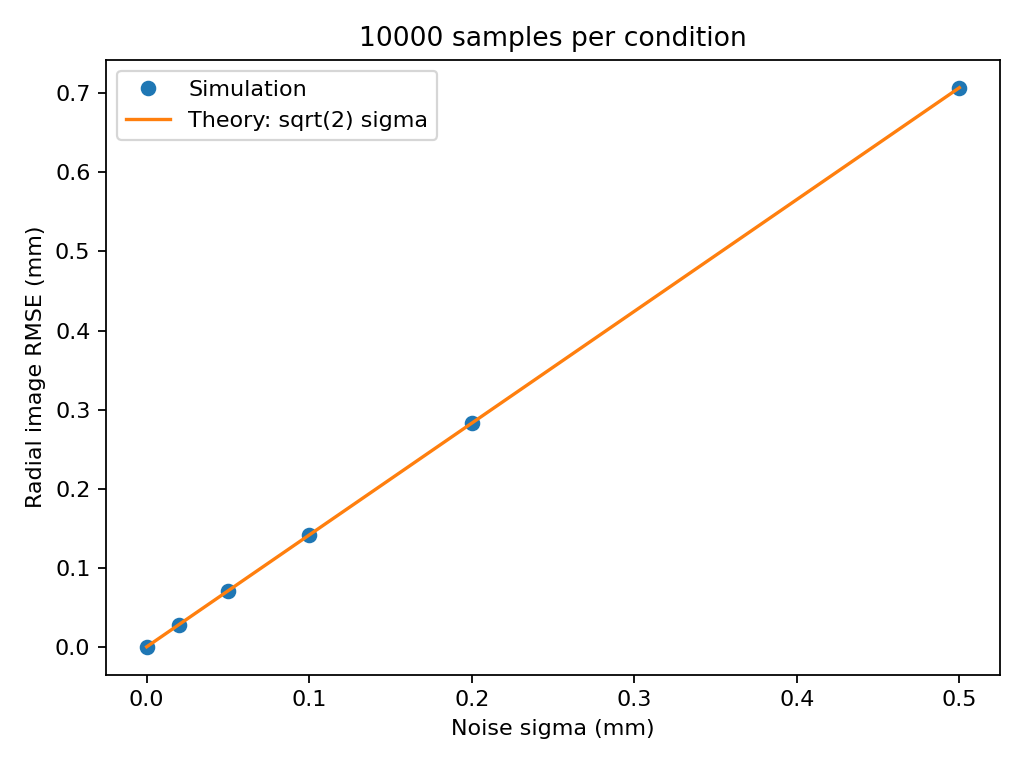
\includegraphics[width=0.78\textwidth]{03_noise.png}
    \caption{Simulated radial RMSE versus theoretical $\sqrt{2}\sigma$ under additive Gaussian noise on image coordinates. Ten thousand Monte-Carlo samples were used for each $\sigma$; a fixed random seed was employed.}
    \label{fig:noise}
\end{figure}

\section{Analysis of Model Fidelity and Dependencies}
\label{sec:analysis}

\subsection{Geometric Properties and Projection Sensitivity}
Equations~\eqref{eq:rotation}--\eqref{eq:fov} determine ideal image positions from target and camera states, provided the target is in front. On a horizontal ground plane, changing pan alone at fixed center and tilt rotates the footprint about the camera's vertical axis; its shape and area remain invariant. Tilt generally changes its shape and area. These are properties of the model, not conclusions that the present count curve alone can establish.

For a downward-facing camera ($\phi=\pi$), height $H=C_z>0$ gives footprint side lengths $aH/\lambda$ and $bH/\lambda$. Therefore
\begin{equation}
A(H)=\frac{abH^2}{\lambda^2},\qquad \frac{dA}{dH}=\frac{2abH}{\lambda^2}.
\label{eq:area}
\end{equation}
This is a special-case analytic prediction of position dependence. It has not yet been checked with a dedicated height-sweep experiment.

Differentiating the projection yields
\begin{equation}
J_q=\frac{\partial p}{\partial q}=\begin{bmatrix}
\lambda/q_z&0&-\lambda q_x/q_z^2\\
0&\lambda/q_z&-\lambda q_y/q_z^2
\end{bmatrix}.
\label{eq:jacobian}
\end{equation}
Thus transverse image sensitivity scales as $\lambda/q_z$, while depth sensitivity also depends on off-axis position. For fixed camera pose, $\partial p/\partial X_T=J_qR_{WC}^T$. With camera and target motion,
\begin{equation}
\dot p=J_q\dot q,\quad
\dot q=R_{WC}^T(\dot X_T-\dot C)-[\omega_C]_\times q,
\end{equation}
where $[\omega_C]_\times=R_{WC}^T\dot R_{WC}$ and $[\omega_C]_\times q=\omega_C\times q$. These derivatives are derived in the report but are not implemented as image-velocity outputs or validated by finite differences in the present code.

\subsection{Noise Statistics and Their Evidence}
For Eq.~\eqref{eq:measurement}, independent coordinate errors imply
\begin{equation}
\mathbb{E}[\|\epsilon\|^2]=2\sigma^2,\qquad
\sqrt{\mathbb{E}[\|\epsilon\|^2]}=\sqrt{2}\sigma.
\end{equation}
A sample RMSE approaches the population value; its finite-sample expectation need not equal that value exactly. The maximum absolute discrepancy across the six existing conditions is approximately $0.000640$ mm. This experiment supports noise statistics only. The geometry checks and the scene plot supply separate, limited evidence for geometric consistency.
\begin{table}[htbp]
\centering
\caption{Existing noise experiment, in image-plane millimeters.}
\begin{tabular}{rrr}\toprule
$\sigma$ & Sample radial RMSE & Population RMS\\\midrule
0&0&0\\0.02&0.028125&0.028284\\0.05&0.070071&0.070711\\
0.10&0.142009&0.141421\\0.20&0.282945&0.282843\\
0.50&0.706817&0.707107\\\bottomrule
\end{tabular}
\end{table}

\subsection{Dependencies Illustrated by the Experiments}
The experiments illustrate the following dependencies required by the midterm project specification:
\begin{itemize}
    \item Sensor orientation (pan) rotates the ground FOV without changing its shape or area under the present planar assumptions and can therefore change the set of targets that produce measurements (Fig.~\ref{fig:pan}).
    \item An environmental obstacle removes targets from the set of available measurements even when they lie inside the geometric FOV (difference between the two curves in Fig.~\ref{fig:pan} and the red markers in Fig.~\ref{fig:scene}).
    \item Target location determines membership in $\mathcal{S}(t)$ (Fig.~\ref{fig:scene}).
\end{itemize}

\subsection{Limitations Relative to the Handout}
The following elements of the handout are not implemented:
\begin{itemize}
    \item Image-plane velocity and numerical Jacobian evaluation (handout Eqs.~6--7). The analytic derivative above has not been added to the code.
    \item Camera kinematic dynamics and the associated inequality constraints (handout Eqs.~10--12 and Table~1).
\end{itemize}
Consequently, the simulation uses prescribed pose sequences rather than dynamically controlled trajectories, and measurements contain only position (not velocity). Height and tilt sweeps, moving targets, independently varied obstacles, lens distortion and real-image validation are also absent. Unknown three-dimensional depth cannot be recovered from a single image point without additional assumptions; ground-plane knowledge is essential for metric back-projection here.

\section{Conclusions}
\label{sec:conclusion}
The current implementation provides a consistent ideal pinhole projection, positive-depth FOV selection, solid-box LOS testing, and additive image-coordinate noise. Existing experiments illustrate pan-dependent target availability and support the assumed noise statistics. Analytic height scaling and projection sensitivity explain additional model dependencies, but their dedicated numerical tests remain incomplete. The highest-priority additions are height/tilt sweeps, target and obstacle variation, and independent geometric validation. Motor control is optional enrichment, not a stated universal requirement of the assignment. The present report is a corrected draft and does not claim a fully validated physical PT sensor.

\begin{thebibliography}{9}
\bibitem{handout}
S.~Ferrari, \textit{Pinhole Camera Model and Field-of-view (FOV)}, 
Course handout, MAE 4810/5810 Robot Perception.

\bibitem{midterm}
\textit{Midterm Project}, MAE 4810/5810 / ECE 4240/5240 Robot Perception.
\end{thebibliography}

\end{document}
